\documentclass[a4paper, 12pt]{article}
\usepackage[utf8]{inputenc}
\usepackage[T1]{fontenc}
\usepackage{lmodern}
\usepackage[croatian, english]{babel}
\usepackage{datetime}
\usepackage{float}
\usepackage{indentfirst}
\usepackage{graphicx}
\usepackage[unicode]{hyperref}
\usepackage[usenames,dvipsnames]{xcolor}
\usepackage{pgfplots}
\usepackage{tikz}
\usepackage{subfiles}
\usepackage{listings}
\usepackage{textcomp}
\usepackage{gensymb}
\usepackage{amsmath}
\usepackage{amsfonts}
\usepackage[colorinlistoftodos]{todonotes}
\usepackage{geometry}
\usepackage{float}
\usepackage{caption}
\usepackage{footnote}
\usepackage[bottom]{footmisc}
\usepackage{lastpage}
\usepackage{multirow}
\usepackage{array}
\usepackage{xcolor}
\usepackage{datetime}
\usepackage[numbers, comma, sort&compress]{natbib}
\usepackage{fancyhdr}
\usepackage{enumitem}
\usepackage{lscape}
\usepackage{pdfpages}
\usepackage{graphicx}

\definecolor{highlight}{RGB}{255,251,204}
\definecolor{DarkGreen}{rgb}{0.0,0.4,0.0} 

\lstdefinestyle{Style1}{
	backgroundcolor=\color{highlight},
	basicstyle=\footnotesize\ttfamily, 
	breakatwhitespace=false, -
	breaklines=true, 
	captionpos=b,
	commentstyle=\usefont{T1}{pcr}{m}{sl}\color{DarkGreen},
	deletekeywords={},
	firstnumber=1,
	frame=single,
	frameround=tttt,
	keywordstyle=\color{Blue}\bf,
	morekeywords={},
	numbers=left,
	numbersep=10pt,
	numberstyle=\tiny\color{black},
	rulecolor=\color{black},
	showstringspaces=false,
	showtabs=false,
	stepnumber=1,
	stringstyle=\color{Purple},
	tabsize=2,
}
\geometry{
    a4paper,
    left=25mm,
    right=25mm,
    top=25mm,
    bottom=25mm
}
\numberwithin{figure}{section}
\numberwithin{equation}{section}
\renewcommand{\listfigurename}{Popis slika}
\renewcommand{\listtablename}{Popis tablica}

\pgfplotsset{compat=1.15}

\begin{document}
\selectlanguage{croatian}

\pagenumbering{arabic}
\setcounter{page}{1}

\newpage
%Naslovna strana
\pagenumbering{gobble}
\iffalse
\begin{flushleft}
	Univerzitet u Sarajevu\\
	Elektrotehnički fakultet\\
	Odsjek za automatiku i elektroniku\\
\end{flushleft}
\fi

\begin{center}

\includegraphics[width=0.1\textwidth]{etf-logo.png}\\
    \Large{\textsc{Univerzitet u Sarajevu}}\\
    \captionsetup{type=figure}
    \large{\textsc{Elektrotehnički fakultet}}\\
    \normalsize\textsc{Odsjek za automatiku i elektroniku}
\end{center}
\vfill

\begin{center}
	\vspace{0.1cm}
	\Large \textbf{Seminarski rad}
	\vspace{0.1cm}
\end{center}

\rule{\textwidth}{0.1mm}

\begin{center}
	\vspace{0.1cm}
	\LARGE \textbf{Proračun struja kratkih spojeva}
	\vspace{0.3cm}
\end{center}

\rule{\textwidth}{0.1mm}

\begin{center}
    \textbf{Dedić Naida, Modrić Emina}\\
   \textit{Predmet: Zaštita i upravljanje elektroenergetskih sistema\\
    Nastavnik: Prof. dr Izudin Džafić, dipl.ing.el}\\
    Akademska godina: 2019/2020.\\
    \vspace{0.5cm}
\end{center}

%Sažetak


\selectlanguage{croatian}

\vfill
\begin{center}
	Sarajevo, januar 2020.
\end{center}

%Sadržaj
\newpage
\clearpage\thispagestyle{empty}

\tableofcontents
\pagenumbering{arabic}
\setcounter{page}{2}

\newpage
\section{Uvod}

Na vodovima elektroenergetske mreže pojavljuju se kvarovi nastali usljed nevremena, grmljavine, snijega, mehaničkog oštećenja nadzemnog voda, proboja izolacije nadzemnog vodiča ili omotača kablova i sl. Prije ponovnog vraćanja u pogon, neophodno je otkloniti dijagnosticirani kvar. \\

Kratki spojevi nastaju usljed premoštavanja izolacije između dijelova električnog postrojenja različitih potencijala. Kvarovi ove vrste čine čak 85\% kvarova u prenosnom sistemu. U skladu s tim, proračun kratkih spojeva kao alat omogućava dobijanje ulaznih parametara za zaštitu, te koordinaciju zaštite. \\

Iz perspektive zaštite od interesa je poznavanje maksimalnih i minimalnih vrijednosti struja na prekidačima snage za vrijeme kvara. Proračun struja kratkih spojeva potrebno je vršiti za sve moguće kombinacije kvarova. Maksimalne struje se koriste za dimenzionisanje prekidača snage, odnosno definisanje njegove prekidne snage, dok se minimalne struje koriste za određivanje praga djelovanja zaštite. Bitno je napomenuti da cijena prekidača snage znatno raste zavisno od vrijednosti prekidne snage. \cite{b0}\\

Generalno, kvar se može predstaviti kao strukturna promjena mreže ekvivalentna razmatranoj mreži sa dodatkom impedanse kvara na odgovarajućem čvoru u mreži. Kroz ovaj rad su razmatrani poprečni kvarovi: jednofazni kratki spoj, dvofazni kratki spoj sa/bez zemlje, te trofazni kratki spoj. 

\subsection{Jednofazni kratki spoj}

Za jednofazni kratki spoj \cite{b1} vrijedi:

\begin{equation}
    V_{a} = 0;
    I_{b} = 0;
    I_{c} = 0;
    \label{eq1}
\end{equation}

Na osnovu vrijednosti iz \ref{eq1} dobiju se sljedeći izrazi za struje u odnosu na čvor $i$ nulte, direktne i inverzne komponente, respektivno:

\begin{equation} 
I^{0}_{i,a} = I^{1}_{i,a}  = I^{2}_{i,a} =\frac{V^{0}_{i}}{Z^{0}_{ii} + Z^{1}_{ii} + Z^{2}_{ii} + 3Z_{f}}
\label{eq2}
\end{equation}

\subsection{Dvofazni kratki spoj sa zemljom}

Za dvofazni kratki spoj sa zemljom \cite{b2} vrijedi:

\begin{equation}
    I_{a} = 0;
    V_{b} = 0;
    V_{c} = 0;
    \label{eq3}
\end{equation}

Na osnovu vrijednosti iz \ref{eq3} dobiju se sljedeći izrazi za struje u odnosu na čvor $i$ nulte, direktne i inverzne komponente, respektivno:

\begin{equation}
I^{1}_{i,a}  = \frac{V^{0}_{i}}{Z^{1}_{ii} + \frac{Z^{2}_{ii}(Z^{0}_{ii} + 3Z_{f})}{Z^{0}_{ii} + Z^{2}_{ii} + 3Z_{f}}}
    \label{eq4}
\end{equation}

\begin{equation}I^{0}_{i,a} = -\frac{V^{0}_{i} - Z^{1}_{ii}I^{1}_{i,a}}{Z^{0}_{ii} + 3Z_{f}}
    \label{eq5}
\end{equation}

\begin{equation}I^{2}_{i,a} =-\frac{V^{0}_{i} - Z^{1}_{ii}I^{1}_{i,a}}{Z^{2}_{ii}}
    \label{eq6}
\end{equation}

\subsection{Dvofazni kratki spoj}

Za dvofazni kratki spoj \cite{b2} vrijedi:

\begin{equation}
    I_{a} = 0;
    V_{b} = V_{c};
    \label{eq7}
\end{equation}

Na osnovu vrijednosti iz \ref{eq7} dobiju se sljedeći izrazi za struje u odnosu na čvor $i$ nulte, direktne i inverzne komponente, respektivno:

\begin{equation}
I^{0}_{i,a}  = 0
    \label{eq8}
\end{equation}

\begin{equation}
I^{1}_{i,a} = -I^{2}_{i,a} = \frac{V^{0}_{i}}{Z^{1}_{ii} + Z^{1}_{ii} + Z_{f}}
    \label{eq9}
\end{equation}

\subsection{Trofazni kratki spoj}

Za trofazni kratki spoj \cite{b2} vrijedi:

\begin{equation}
    I_{a} + I_{b} +I_{c} = 0;
    V_{a} = V_{b} = V_{c};
    \label{eq10}
\end{equation}
Kvar je simetričan, pa se razmatra samo pozitivna komponenta sistema. 
Na osnovu vrijednosti iz \ref{eq3} dobiju se sljedeći izrazi za struje u odnosu na čvor $i$ nulte, direktne i inverzne komponente, respektivno:

\begin{equation}
I^{1}_{i,a}  = \frac{V^{0}_{i}}{Z_{ii} + Z_{f}}
    \label{eq11}
\end{equation}

\begin{equation}I^{0}_{i,a} = I^{2}_{i,a} = 0
    \label{eq12}
\end{equation}













\newpage
\section{Dizajn}
U radu su vršeni proračuni kratkih spojeva za tri različita elektroenergetska sistema. Za svaki sistem kreiran je odgovarajući grafički korisnički interfejs (GUI) aplikacije za proračun kratkih spojeva, pa se time svaki sistem može posmatrati odvojeno. Na slici \ref{A1} prikazana je shema mreže prvog elektroenergetskog sistema, a kreirani GUI za taj sistem se među kodovima može pronaći pod nazivom gui.

\begin{center}
    \captionsetup{type=figure}
    \begin{center}
        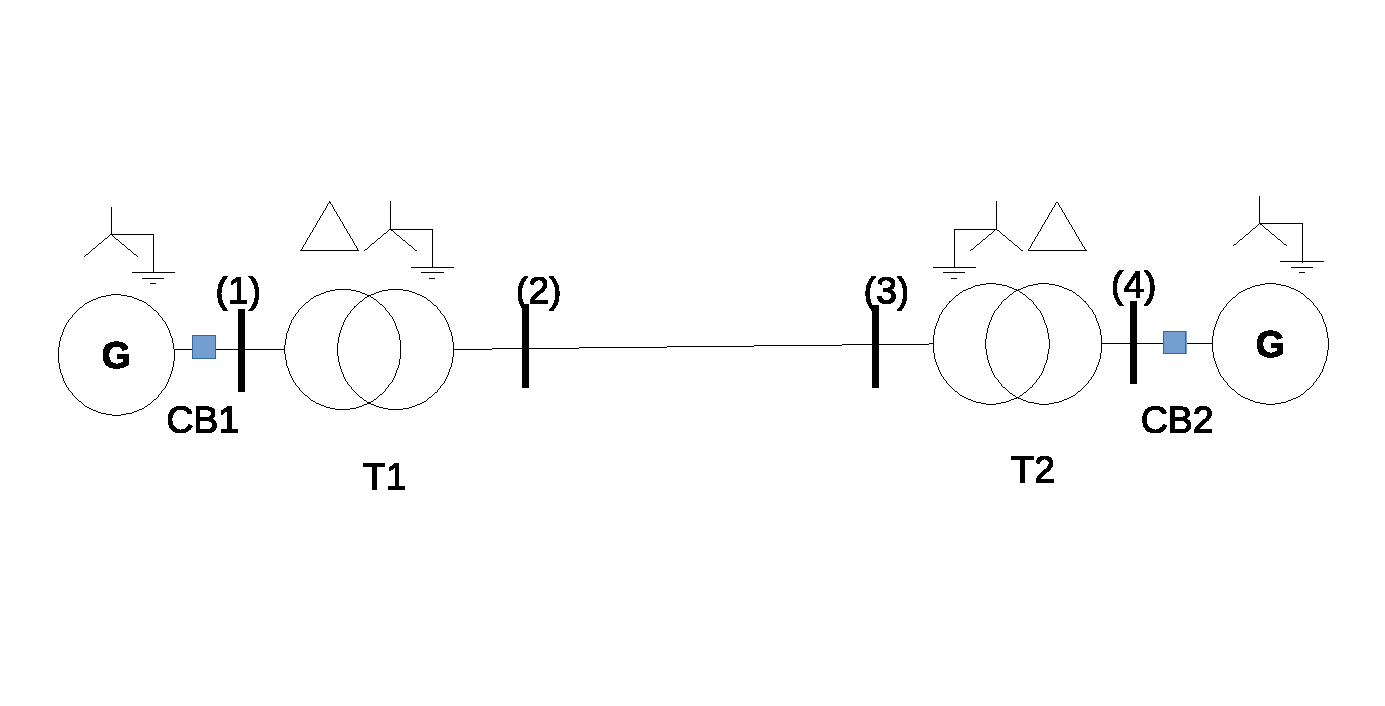
\includegraphics[width=\textwidth]{slike/shema1.eps}
        \caption{Shema za mrežu 1}
        \label{A1}
    \end{center}
\end{center}

Shema za drugi razmatrani elektroenergetski sistem prikazana je na slici \ref{A2}, a odgovarajući GUI kreiran za taj sistem ima naziv gui\_shema2.

\begin{center}
    \captionsetup{type=figure}
    \begin{center}
        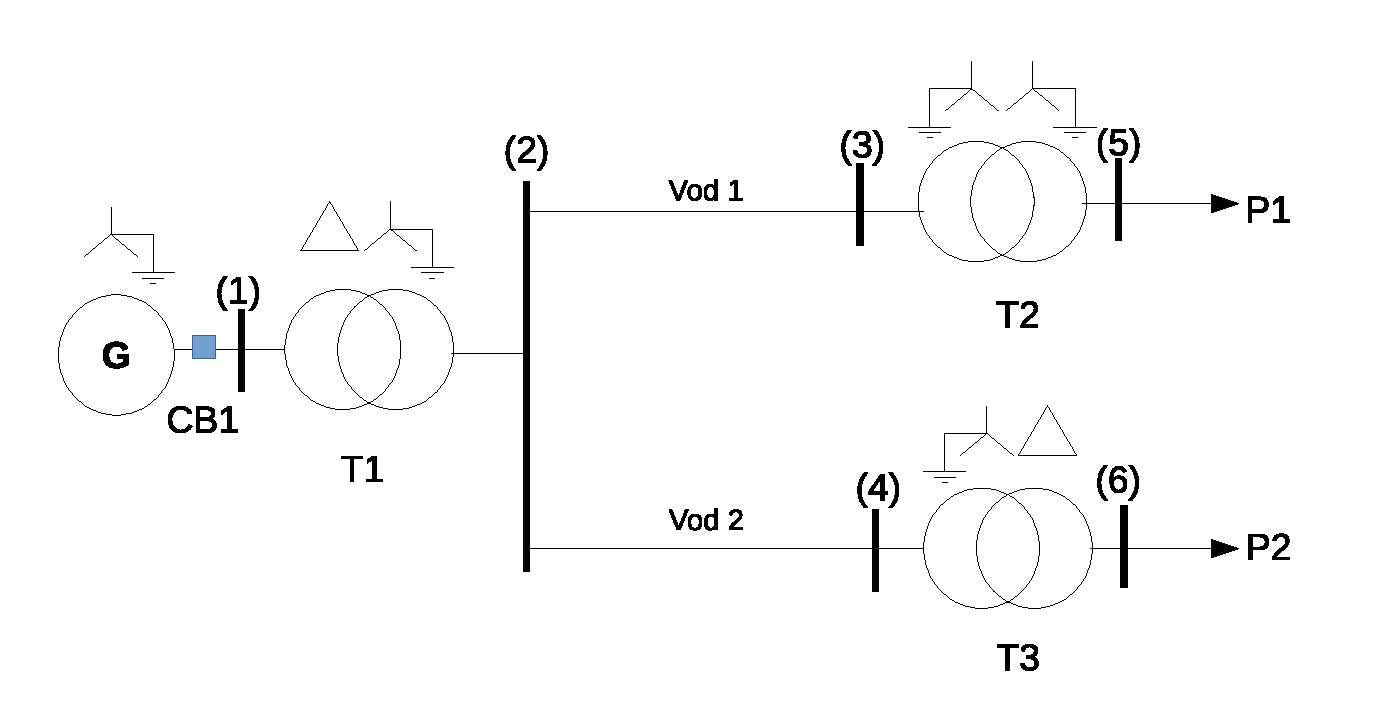
\includegraphics[width=\textwidth]{slike/shema2.eps}
        \caption{Shema za mrežu 2}
        \label{A2}
    \end{center}
\end{center}

Shema treće elektroenergetske mreže razmatrane u ovom radu prikazana je na slici \ref{A3}, a odgovarajući GUI kreiran za taj sistem ima naziv gui\_shema3.

\begin{center}
    \captionsetup{type=figure}
    \begin{center}
        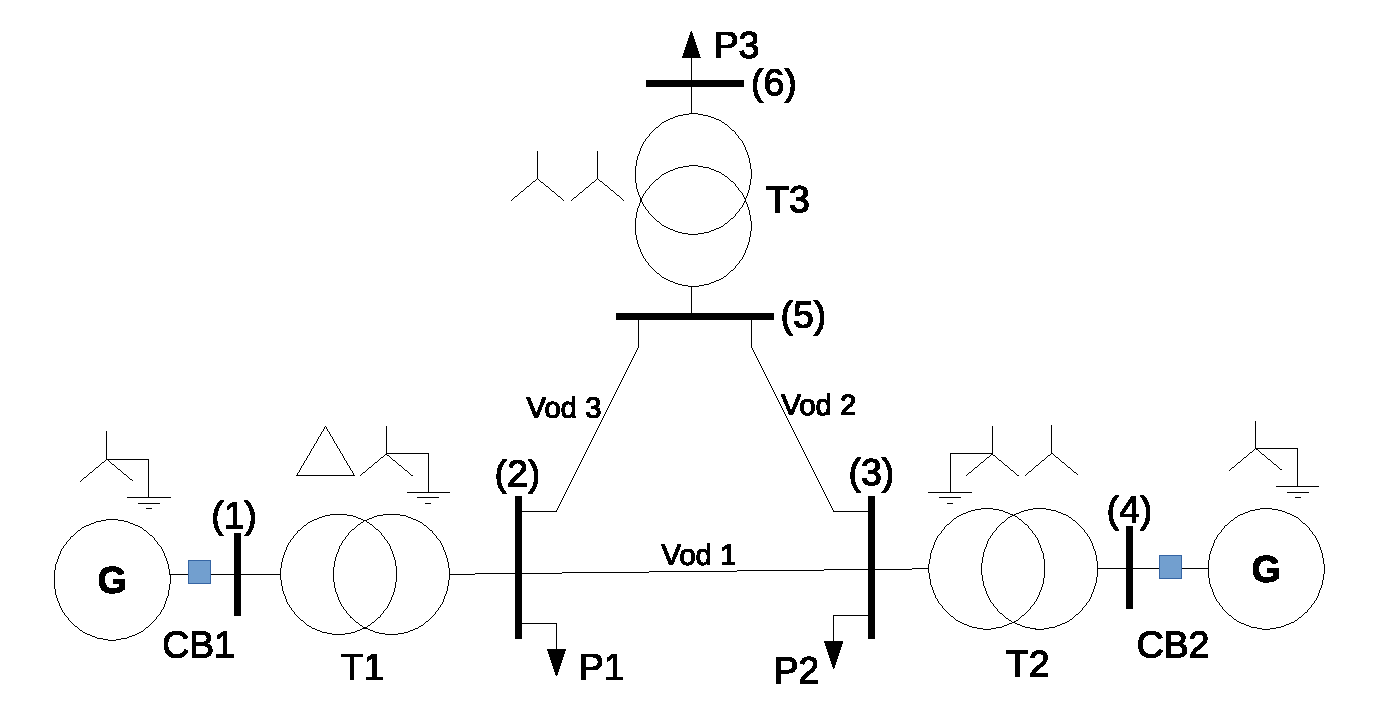
\includegraphics[width=\textwidth]{slike/shema3.eps}
        \caption{Shema za mrežu 3}
        \label{A3}
    \end{center}
\end{center}

Na slici \ref{E1} je prikazan GUI aplikacije za prvi elektroenergetski sistem (koji ima odgovarajuću shemu broj 1). 

\begin{center}
    \captionsetup{type=figure}
    \begin{center}
        \includegraphics[width=\textwidth]{slike/guishema1.eps}
        \caption{GUI aplikacije za proračun kratkih spojeva za shemu 1}
        \label{E1}
    \end{center}
\end{center}

U gornjem dijelu grafičkog korisničkog interfejsa koji je prikazan na slici \ref{E2} omogućen je unos parametara mreže elektroenergetskog sistema čija je mreža prikazana u srednjem dijelu grafičkog interfejsa aplikacije (vidi se na slici \ref{E1}). 

\begin{center}
    \captionsetup{type=figure}
    \begin{center}
        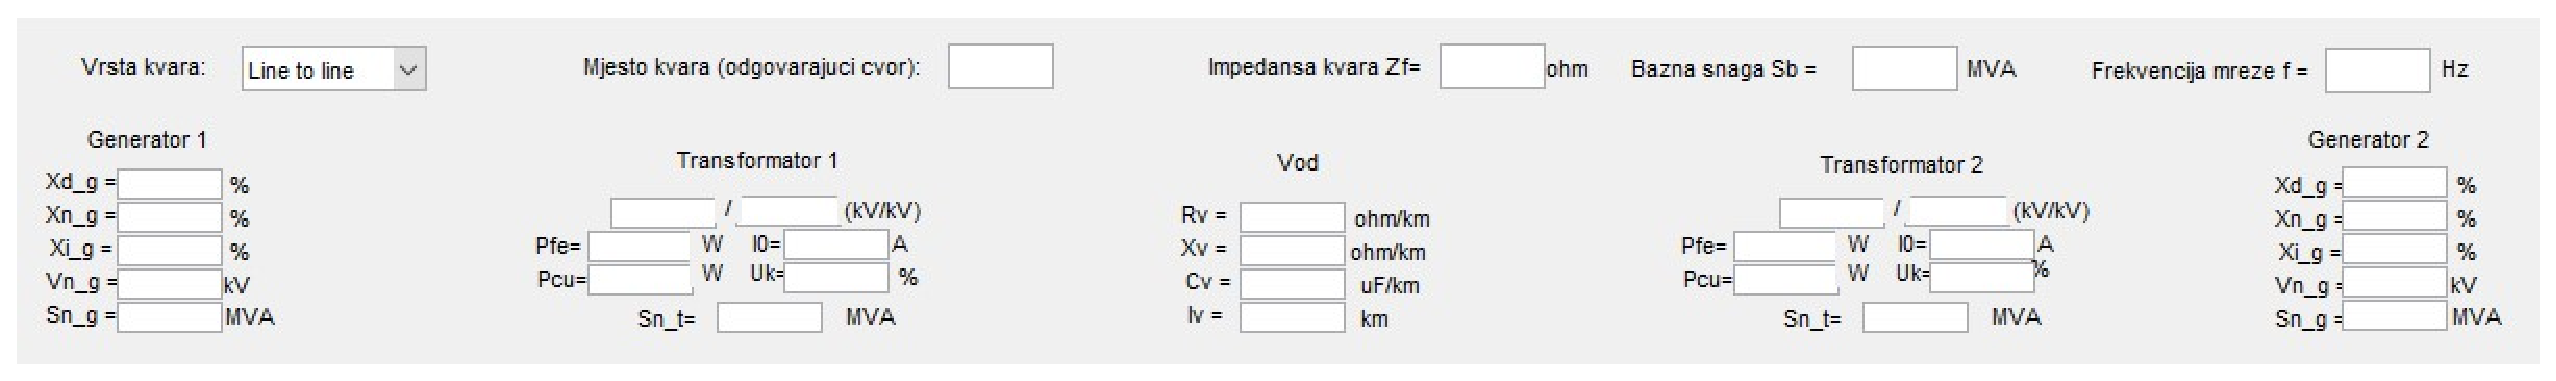
\includegraphics[width=\textwidth]{slike/shema1gui_gornji.eps}
        \caption{Dio GUI-a za unos parametara mreže}
        \label{E2}
    \end{center}
\end{center}

Vrsta kvara koji se proračunava se bira iz pop-up menija nazvanog $\textit{Vrsta kvara}$. Dalje se unose mjesto kvara koje predstavlja odgovarajući čvor na shemi mreže sistema, impedansa kvara $Z_{f}$, frekvencija mreže $f$ i bazna snaga $S_{b}$ u odnosu na koju se vrši per-unit proračun. Nakon ovoga, unose se odgovarajući parametri elemenata mreže, kao što su generatori, potrošači, transformatori i vodovi. Za ove elemente unose se njihovi nominalni naponi, snage i parametri potrebni za proračunavanje njihovih odgovarajućih impedansi.\\

Nakon što su uneseni svi parametri mreže elektroenergetskog sistema, pritiskom na dugme $\textit{Racunaj}$ vrši se proračun svih struja i napona u mreži nakon kvara. Na kraju se računaju struje na svim prekidačima snage u mreži i ispisuju se na predviđeno mjesto prikazano na slici \ref{E3}. Za svaki prekidač snage se odvojeno ispisuju vrijednosti a, b i c faznih komponenti struje koja teče odgovarajućom granom.

\begin{center}
    \captionsetup{type=figure}
    \begin{center}
        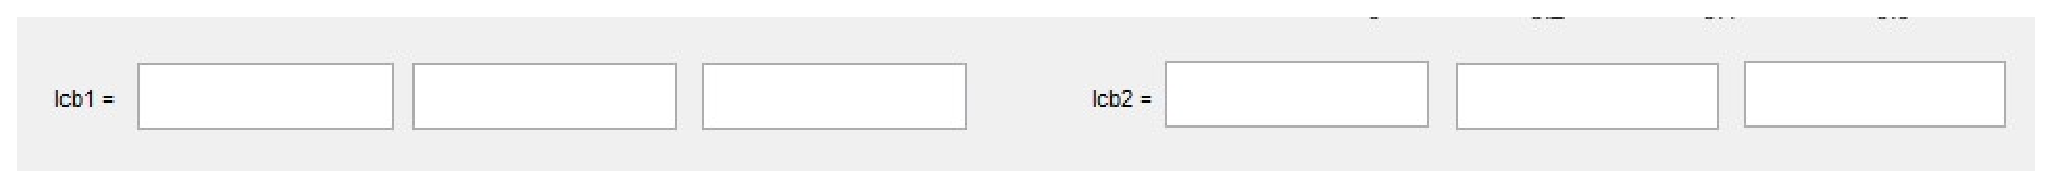
\includegraphics[width=\textwidth]{slike/shema1gui_donji.eps}
        \caption{Dio GUI-a za ispis struja na prekidačima snage}
        \label{E3}
    \end{center}
\end{center}

Na srednjem dijelu grafičkog korisničkog interfejsa pored sheme mreže elektroenergetskog sistema vidi se i jedan prazan prozor. Na tom dijelu GUI-a će se nakon proračunavanja struja na prekidačima snage prikazivati vektorski dijagrami struja na prekidačima snage.\\

Za preostala dva razmatrana elektroenergetska sistema grafički korisnički interfejs aplikacije je skoro isti, jedina razlika je u tome što je shema sistema drugačija te se samim time unose drugačiji parametri u GUI, a koji su odgovarajući za razmatranu shemu. GUI prikazi za preostale dvije mreže se svode na isto, te ih stoga nije potrebno zasebno razmatrati.\\






















\newpage
\section{Implementacija}

\subsection{Konvertovanje svih vrijednosti u per unit}

Zone sa istim nazivnim naponom određuju se na način da se izbace transformatori, a potom svakoj galvanski spojenoj oblasti dodijelimo linijski napon u $kV$. Transformator se priključuje oblasti zavisno od naponskog nivoa na kojem su bili postavljeni mjerni instrumenti tokom izvođenja eksperimenata praznog hoda i kratkog spoja. Na razmatranim shemama pomenuti eksperimenti su vršeni na naponskom nivou sa strane odgovarajućeg voda. \\

Na osnovu zadane bazne snage $S_{b}$ potrebno je konvertovati snage svih potrošača/generatora u per unit sistem. Zatim, za svaku oblast k je potrebno proračunati baznu struju $I_{bk}$ i baznu impedansu $Z_{bk}$.
U per unit sistem potrebno je prevesti i sve impedanse unutar razmatranog sistema i napone svakog od čvorova, i to dijeljenjem odgovarajućim baznim impedansama i vrijednostima napona baznih nivoa, respektivno. \\

Listing $\textit{Matlab}$ koda kojim je implementirana konverzija parametara sistema u per unit sistem prikazan je u nastavku.

\lstinputlisting[language=python,style=Style1]{perUnit.m}

\subsection{Određivanje napona prije kvara za svaki čvor}

S ciljem određivanja vrijednosti napona prije kvara za svaki čvor (slack, PV i PQ čvorovi) koristimo relaciju \ref{J1}. Pri tome, za simetričan sistem vrijedi $V^{(pre)}_{0}=V^{(pre)}_{2}=0$.

\begin{equation}
    Y^{(pre)}_{1}V^{(pre)}_{1} = I^{(pre)}_{1}
    \label{J1}
\end{equation}

U kodu u nastavku prikazan je način implementacije razmatranog proračuna. Matrica impedansi prije kvara određena je manuelno - inspekcijom mreže.

\lstinputlisting[language=python,style=Style1]{naponiPrijeKvara.m}

\subsection{Određivanje  Thevenin-ovog ekvivalentnog napona na mjestu kvara}

Thevenin-ov ekvivalentni napon na mjestu kvara jednak je naponu prije kvara na čvoru na kojem se kvar desio (relacija \ref{J2}).

\begin{equation}
    u^{(Th)}_{1}=V^{(Th)}_{1}(k)
    \label{J2}
\end{equation}

\lstinputlisting[language=python,style=Style1]{naponThevenen.m}

\subsection{Formiranje matrica $Y^{(f)}_{0}, Y^{(f)}_{1}, Y^{(f)}_{2}$}

Pri kreiranju matrica admitansi $Y^{(f)}_{0}, Y^{(f)}_{1}, Y^{(f)}_{2}$ vodovi i transformatori aproksimirani su odgovarajućim pi parametrima četveropola. Transformatori su predstavljeni impedansom u poprečnoj grani  $Z_{s}$ ,koja se određuje uz pomoć parametara eksperimenta kratkog spoja $P_{cu}$ i $U_{k}$, i impedansom u otočnim granama $Z_{x}$, koja se određuje uz pomoć parametara eksperimenta praznog hoda $P_{fe}$ i $I_{0}$. Vodovi su predstavljeni impedansom u poprečnoj grani koja je utvrđena uz pomoć podužnih parametara voda i dužine voda, te impedansom u otočnim granama čija se vrijednost računa uz pomoć kapacitivne komponente voda.

Mreža za pozitivnu komponentu $(1)$ topološki je ekvivalentna mreži negativne $(2)$ komponente. Vrijednosti impedansi pozitivne i negativne komponente različite su samo za rotacione mašine, pa se u skladu s tim odgovarajuće matrice impedansi razlikuju samo po vrijednosti impedanse generatora. \\

Pojedine transformatorske konekcije unose prekid nulte komponente $(0)$, pa je prije formiranja matrice $Y^{(f)}_{0}$ potrebno nacrtati mrežu uz uvažavanje transformatorskih konekcija i vrijednosti impedansi nulte komponente za generatore i vodove. \\

\lstinputlisting[language=python,style=Style1]{matriceYfault.m}

Bitno je napomenuti da kod sheme 2 i sheme 3 postoji mogućnost da matrica $Y^{(f)}_{0}$ bude singularna (zavisno od parametara unesenih za potrošače), što matematički predstavlja problem za nastavak proračuna. U tom slučaju, potrebno je proračunati matrice $Y^{(f)}_{0_i}$ za svaki od i impedantno odvojenih dijelova kola, a potom posredstvom njih formirati matricu $Z^{(f)}_{0}$. Način rješavanja pomenutog problema za ove dvije sheme prikazan je u nastavku. \\

\lstinputlisting[language=python,style=Style1]{singularna_shema2.m}
\lstinputlisting[language=python,style=Style1]{singularna_shema3.m}

\subsection{Ekvivalentna Thevenin-ova impedansa na mjestu kvara $z^{(f)}_{0}, z^{(f)}_{1}, z^{(f)}_{2}$}

\lstinputlisting[language=python,style=Style1]{impedansaThevenen.m}

\subsection{Nalaženje struja kvara $i^{(f)}_{0}, i^{(f)}_{1}, i^{(f)}_{2}$ korištenjem modela kvara}

Da bismo odredili struje kvara, potrebno je prvenstveno definisati vrstu kvara. Listing $\textit{Matlab}$ kodova zavisno od vrste kvara prikazan je u nastavku.

\subsubsection{Jednofazni kratki spoj sa zemljom}

\lstinputlisting[language=python,style=Style1]{line_to_ground1.m}

\subsubsection{Dvofazni kratki spoj}

\lstinputlisting[language=python,style=Style1]{line_to_line1.m}

\subsubsection{Dvofazni kratki spoj sa zemljom}

\lstinputlisting[language=python,style=Style1]{double_line_to_ground1.m}

\subsubsection{Trofazni kratki spoj}

\lstinputlisting[language=python,style=Style1]{three_phase1.m}

\subsection{Kompenzacioni naponi i naponi u toku kvara}

Kompenzacioni naponi i naponi u toku kvara određeni su za svaki čvor i svaku od komponenti (nulta, direktna, inverzna). Pri proračunu u obzir je uzeta i mogućnost singularnosti matrice $Y^{(f)}_{0}$. \\

\lstinputlisting[language=python,style=Style1]{naponi.m}

\subsection{Proračun struja kroz prekidače snaga}

Listing koda za proračun struja kroz prekidače snaga $CB1$ i $CB2$ za shemu 1 prikazan je u nastavku. \\

\lstinputlisting[language=python,style=Style1]{shema1_finalno.m}













\newpage
\section{Testiranje}

U ovom poglavlju rada bit će pojašnjeno testiranje aplikacije za proračunavanje struja kratkih spojeva posredstvom GUI-a. Testiranje će biti odvojeno izvršeno za sve tri mreže koje su obrađene u aplikaciji.

\subsection{Mreža 1}

Za testiranje mreže potrebno je unijeti parametre elemenata mreže u odgovarajuća polja na grafičkom korisničkom interfejsu.  Na slici \ref{E4} prikazane su vrijednosti unesenih parametara za elemente iz mreže. 

\begin{center}
    \captionsetup{type=figure}
    \begin{center}
        \includegraphics[width=\textwidth]{slike/shema1_testiranje.eps}
        \caption{GUI - testiranje sheme 1}
        \label{E4}
    \end{center}
\end{center}

Testiranje će biti vršeno za sve četiri vrste kvarova, koji će se tokom testiranja birati iz pop-up menija. Testiranje kvarova je vršeno na čvoru 3 sa impedansom kvara $4+1i$, a frekvencija mreže je $50Hz$. Vrijednosti parametara za generatore, potrošače, transformatore i vodove se vide na slici \ref{E4}.

\subsection{Mreža 2}

Na mreži 2 tokom testiranja za čvor na kojem se desio kvar izabran je čvor 4, a impedansa kvara iznosi $4+1i$. Frekvencija mreže je $50Hz$. Vrijednosti parametara za generatore, potrošače, transformatore i vodove su postavljene na vrijednosti čiji red veličine ima fizikalni smisao i mogu se vidjeti na slici \ref{E5}. Pored ovoga, izvršit će se i testiranje u slučaju kada je linija prema potrošaču prekinuta. (U poglavlju 3 je već spomenuto kako se u tom slučaju pojavljuje singularna matrica). U ovom slučaju za cilj testiranja prekinuta je linija prema potrošaču 1, pri čemu je promatran dvofazni kratak spoj sa zemljom.

\begin{center}
    \captionsetup{type=figure}
    \begin{center}
        \includegraphics[width=\textwidth]{slike/shema2_testiranje.eps}
        \caption{GUI - testiranje sheme 2}
        \label{E5}
    \end{center}
\end{center}

\subsection{Mreža 3}

Na mreži 3 tokom testiranja za čvor na kojem se desio kvar izabran je čvor 3, a impedansa kvara ponovno iznosi $4+1i$. Frekvencija mreže je $50Hz$. Vrijednosti parametara za generatore, potrošače, transformatore i vodove su postavljene na vrijednosti čiji red veličine ima fizikalni smisao i mogu se vidjeti na slici \ref{E6}. Pored ovoga, ponovno će se izvršiti i testiranje u slučaju kada je linija prema potrošaču prekinuta. U ovom slučaju za cilj testiranja prekinuta je linija prema potrošaču 3, pri čemu je promatran dvofazni kratak spoj sa zemljom.

\begin{center}
    \captionsetup{type=figure}
    \begin{center}
        \includegraphics[width=\textwidth]{slike/shema3_testiranje.eps}
        \caption{GUI - testiranje sheme 3}
        \label{E6}
    \end{center}
\end{center}





























\newpage
\section{Rezultati}

U ovom poglavlju bit će dati rezultati testiranja aplikacije za proračun kratkih spojeva za slučajeve date u poglavlju 4.

 \subsection{Mreža 1}
 Za mrežu 1 rezultati izvršenih testiranja dati su na slikama \ref{E7}, \ref{E8}, \ref{E9} i \ref{E10} koji redom odgovaraju jednofaznom kratkom spoju sa zemljom, dvofaznom kratkom spoju, dvofaznom kratkom spoju sa zemljom te trofaznom kratkom spoju, respektivno.
 
 \begin{center}
    \captionsetup{type=figure}
    \begin{center}
        \includegraphics[width=\textwidth]{slike/shema1_rezultati_linetoground.eps}
        \caption{GUI - rezultati jednofaznog kratkog spoja sa zemljom za shemu 1}
        \label{E7}
    \end{center}
\end{center}

\begin{center}
    \captionsetup{type=figure}
    \begin{center}
        \includegraphics[width=\textwidth]{slike/shema1_rezultati_linetoground.eps}
        \caption{GUI - rezultati dvofaznog kratkog spoja za shemu 1}
        \label{E8}
    \end{center}
\end{center}

\begin{center}
    \captionsetup{type=figure}
    \begin{center}
        \includegraphics[width=\textwidth]{slike/shema1_rezultati_linetoground.eps}
        \caption{GUI - rezultati dvofaznog kratkog spoja sa zemljom za shemu 1}
        \label{E9}
    \end{center}
\end{center}

\begin{center}
    \captionsetup{type=figure}
    \begin{center}
        \includegraphics[width=\textwidth]{slike/shema1_rezultati_linetoground.eps}
        \caption{GUI - rezultati trofaznog kratkog spoja za shemu 1}
        \label{E10}
    \end{center}
\end{center}




\subsection{Mreža 2}
 Za mrežu 2 rezultati izvršenih testiranja kada su svi potrošači priključeni na mrežu dati su na slikama \ref{E11}, \ref{E12}, \ref{E13} i \ref{E14} koji redom odgovaraju jednofaznom kratkom spoju sa zemljom, dvofaznom kratkom spoju, dvofaznom kratkom spoju sa zemljom te trofaznom kratkom spoju, respektivno.
 
 \begin{center}
    \captionsetup{type=figure}
    \begin{center}
        \includegraphics[width=\textwidth]{slike/shema2_rezultati_linetoground.eps}
        \caption{GUI - rezultati jednofaznog kratkog spoja sa zemljom za shemu 2}
        \label{E11}
    \end{center}
\end{center}

\begin{center}
    \captionsetup{type=figure}
    \begin{center}
        \includegraphics[width=\textwidth]{slike/shema2_rezultati_linetoground.eps}
        \caption{GUI - rezultati dvofaznog kratkog spoja za shemu 2}
        \label{E12}
    \end{center}
\end{center}

\begin{center}
    \captionsetup{type=figure}
    \begin{center}
        \includegraphics[width=\textwidth]{slike/shema2_rezultati_linetoground.eps}
        \caption{GUI - rezultati dvofaznog kratkog spoja sa zemljom za shemu 2}
        \label{E13}
    \end{center}
\end{center}

\begin{center}
    \captionsetup{type=figure}
    \begin{center}
        \includegraphics[width=\textwidth]{slike/shema2_rezultati_linetoground.eps}
        \caption{GUI - rezultati trofaznog kratkog spoja za shemu 2}
        \label{E14}
    \end{center}
\end{center}

U slučaju kada je linija koja povezuje potrošača P1 sa mrežom prekinuta, rezultati testiranja su prikazani na slici \ref{E15}

\begin{center}
    \captionsetup{type=figure}
    \begin{center}
        \includegraphics[width=\textwidth]{slike/shema2_rezultati_sing.eps}
        \caption{GUI - rezultati kada je odspojen potrošač P1 za shemu 2}
        \label{E15}
    \end{center}
\end{center}

\subsection{Mreža 3}
 Za mrežu 3 rezultati izvršenih testiranja kada su svi potrošači priključeni na mrežu dati su na slikama \ref{E16}, \ref{E17}, \ref{E18} i \ref{E19} koji redom odgovaraju jednofaznom kratkom spoju sa zemljom, dvofaznom kratkom spoju, dvofaznom kratkom spoju sa zemljom te trofaznom kratkom spoju, respektivno.
 
 \begin{center}
    \captionsetup{type=figure}
    \begin{center}
        \includegraphics[width=\textwidth]{slike/shema3_rezultati_doublelinetoground.eps}
        \caption{GUI - rezultati jednofaznog kratkog spoja sa zemljom za shemu 3}
        \label{E16}
    \end{center}
\end{center}

\begin{center}
    \captionsetup{type=figure}
    \begin{center}
        \includegraphics[width=\textwidth]{slike/shema3_rezultati_linetoground.eps}
        \caption{GUI - rezultati dvofaznog kratkog spoja za shemu 3}
        \label{E17}
    \end{center}
\end{center}

\begin{center}
    \captionsetup{type=figure}
    \begin{center}
        \includegraphics[width=\textwidth]{slike/shema3_rezultati_linetoground.eps}
        \caption{GUI - rezultati dvofaznog kratkog spoja sa zemljom za shemu 3}
        \label{E18}
    \end{center}
\end{center}

\begin{center}
    \captionsetup{type=figure}
    \begin{center}
        \includegraphics[width=\textwidth]{slike/shema3_rezultati_linetoground.eps}
        \caption{GUI - rezultati trofaznog kratkog spoja za shemu 3}
        \label{E19}
    \end{center}
\end{center}

U slučaju kada je linija koja povezuje potrošača P3 sa mrežom prekinuta, rezultati testiranja su prikazani na slici \ref{E20}

\begin{center}
    \captionsetup{type=figure}
    \begin{center}
        \includegraphics[width=\textwidth]{slike/shema3_rezultati_sing.eps}
        \caption{GUI - rezultati kada je odspojen potrošač P3 za shemu 3}
        \label{E20}
    \end{center}
\end{center}

















\newpage
\section{Zaključak i mogućnosti za dalji rad}

U radu su vršeni proračuni kratkih spojeva za tri različita elektroenergetska sistema, pri čemu je za svaki od sistema moguće odabrati jednofazni kratki spoj, dvofazni kratki spoj, dvofazni kratki spoj sa zemljom, te trofazni kratki spoj kao vrstu kvara. \\

Za svaki od sistema kreiran je odgovarajući grafički korisnički interfejs (GUI), koji omogućava unošenje parametara dijelova elektroenergetske distributivne mreže od interesa: generatora, transformatora, vodova, te potrošača. U okviru GUI-a kao rezultat se dobijaju proračunate struje kroz prekidače snage, kao i dijagram - fazorski prikaz pomenutih struja. Cilj proračunavanja parametara jeste pojednostavljivanje određivanja minimalnih specifikacija prekidača snage koji može zadovoljiti uslove rada, a da je pri tome sama mreža zaštićena. \\

Bitno je napomenuti da u stvarnosti postoji opcija prekida linije ka potrošaču. U tom slučaju, kroz implementaciju GUI-a za shemu 2 i za shemu 3 omogućen je dopunski proračun koji koristi činjenicu da su u zamjenskoj shemi nulte komponente dijelovi iste impedantno razdvojeni. \\

Kao prijedlog unapređivanja GUI-a i daljeg rada na aplikaciji potrebno je razmotriti mogućnost dinamičkog dodavanja sheme elektroenergetske mreže koju želimo razmatrati, umjesto trenutno korištenih statičkih shema. Time bi se upotrebljivost napravljene aplikacije digao na viši nivo, te omogućio širi spektar upotrebe.



\newpage
\begin{thebibliography}{00}

\bibitem{b0} I. Džafić, predavanja na predmetu: Zaštita i upravljanje elektroenergetskih sistema, Univerzitet u Sarajevu, ak. 2019/2020.

\bibitem{b1} I. Džafić, E. Halilović, E. Karamehmedović, Introduction to
Power System Analysis, International University of Sarajevo, 2019.

\bibitem{b2} E. Orešković, Kratki spoj u distribucijskim mrežama, Sveučilište u Rijeci, Tehnički fakultet, 2016.


\end{thebibliography}






\end{document}
